\documentclass[tikz,border=4pt]{standalone}
\usepackage{tikz}
\usetikzlibrary{calc}

% ── Colours ──────────────────────────────────────────────────────────────
\definecolor{bigcirclefill}{RGB}{230,241,251}   % light blue
\definecolor{bigcircleborder}{RGB}{55,138,221}  % mid blue
\definecolor{smlcirclefill}{RGB}{234,243,222}   % light green
\definecolor{smlcircleborder}{RGB}{59,109,17}   % mid green
\definecolor{colP1}{RGB}{24,95,165}             % dark blue  – p1, p1'
\definecolor{colP2}{RGB}{163,45,45}             % dark red   – p2
\definecolor{colQ2}{RGB}{15,110,86}             % dark green – q2
\definecolor{colP2prime}{RGB}{133,79,11}        % dark amber – p2'

% ── Shared style keys ────────────────────────────────────────────────────
\tikzset{
  simplex/.style   = {draw, thick, fill=white},
  bigcirc/.style   = {draw=bigcircleborder, fill=bigcirclefill,
                       fill opacity=0.55, dashed, thick},
  smlcirc/.style   = {draw=smlcircleborder, fill=smlcirclefill,
                       fill opacity=0.60, dashed, thick},
  ghostcirc/.style = {draw=bigcircleborder, dashed, opacity=0.30},
  theline/.style   = {draw=gray!60, dashed, thin},
  dot/.style       = {circle, inner sep=0pt, minimum size=5pt, fill=#1},
}

% ── Coordinates (computed in natural units, triangle A=(0,0) B=(4,0) C=(2,3)) ──
% p1   = (1.40, 0.70)
% p2   = (2.20, 1.80)
% q2   = (1.929, 1.428)   — big-circle boundary on segment p1→p2
% p1'  = (1.665, 1.064)   — midpoint(p1, q2), centre of small circle
% p2'  = (1.165, 0.377)   — other side of p1, inside big circle

\begin{document}

% ════════════════════════════════════════════════════════════════════
% Three sub-figures side by side; each figure is 4 units wide.
% Figures are separated by 1.2 units of whitespace.
% ════════════════════════════════════════════════════════════════════
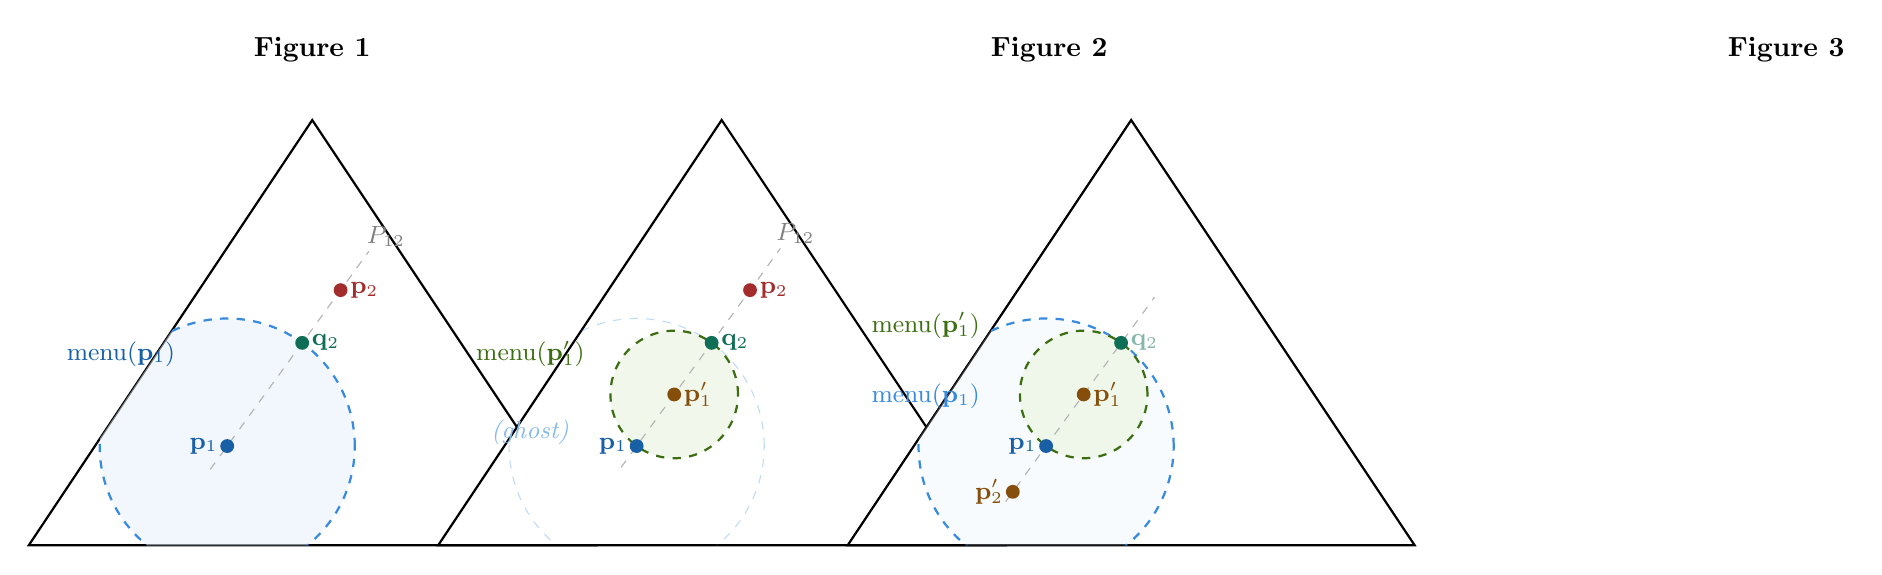
\begin{tikzpicture}[x=1.8cm, y=1.8cm]

  % ── horizontal offsets for the three figures ──
  \def\dxb{5.2}   % offset for Figure 2
  \def\dxc{10.4}  % offset for Figure 3

  % ──────────────────────────────────────────────
  %  FIGURE CAPTIONS
  % ──────────────────────────────────────────────
  \node[font=\bfseries] at (2,      3.5) {Figure 1};
  \node[font=\bfseries] at (2+\dxb, 3.5) {Figure 2};
  \node[font=\bfseries] at (2+\dxc, 3.5) {Figure 3};

  % ══════════════════════════════════════════════
  %  FIGURE 1
  %  Triangle, big circle, line P12, p1, p2, q2
  % ══════════════════════════════════════════════
  \begin{scope}

    % simplex triangle
    \draw[simplex] (0,0) -- (4,0) -- (2,3) -- cycle;

    % big circle, clipped to triangle
    \begin{scope}
      \clip (0,0) -- (4,0) -- (2,3) -- cycle;
      \draw[bigcirc] (1.4, 0.7) circle (0.9);
    \end{scope}

    % line P12 (extended slightly, stays inside triangle)
    \draw[theline] (1.280, 0.535) -- (2.400, 2.075);

    % points
    \node[dot=colP1]  at (1.4,  0.7)   {};
    \node[dot=colP2]  at (2.2,  1.8)   {};
    \node[dot=colQ2]  at (1.929,1.428) {};

    % labels
    \node[left,  font=\small, colP1] at (1.4,  0.7)    {$\mathbf{p}_1$};
    \node[right, font=\small, colP2] at (2.2,  1.8)    {$\mathbf{p}_2$};
    \node[right, font=\small, colQ2] at (1.929,1.428)  {$\mathbf{q}_2$};

    % circle label
    \node[font=\small, colP1, align=center]
      at (0.65, 1.35) {$\mathrm{menu}(\mathbf{p}_1)$};

    % line label
    \node[font=\small, gray]
      at (2.52, 2.18) {$P_{12}$};

  \end{scope}

  % ══════════════════════════════════════════════
  %  FIGURE 2
  %  Same triangle + ghost big circle + small circle
  %  Line through p1' and p2 passing through q2
  % ══════════════════════════════════════════════
  \begin{scope}[xshift=\dxb cm]

    % simplex triangle
    \draw[simplex] (0,0) -- (4,0) -- (2,3) -- cycle;

    % ghost big circle
    \begin{scope}
      \clip (0,0) -- (4,0) -- (2,3) -- cycle;
      \draw[ghostcirc] (1.4, 0.7) circle (0.9);
    \end{scope}

    % small circle (r = 0.45, centred at p1')
    \begin{scope}
      \clip (0,0) -- (4,0) -- (2,3) -- cycle;
      \draw[smlcirc] (1.665, 1.064) circle (0.45);
    \end{scope}

    % line through p1' and p2 (extended, passes through q2)
    \draw[theline] (1.290, 0.549) -- (2.414, 2.094);

    % points
    \node[dot=colP1]           at (1.4,   0.7)   {};   % p1 on boundary of small circle
    \node[dot=colP2]           at (2.2,   1.8)   {};   % p2
    \node[dot=colQ2]           at (1.929, 1.428) {};   % q2 on boundary of small circle
    \node[dot=colP2prime]      at (1.665, 1.064) {};   % p1' centre of small circle

    % labels
    \node[left,  font=\small, colP1]     at (1.4,   0.7)   {$\mathbf{p}_1$};
    \node[right, font=\small, colP2]     at (2.2,   1.8)   {$\mathbf{p}_2$};
    \node[right, font=\small, colQ2]     at (1.929, 1.428) {$\mathbf{q}_2$};
    \node[right, font=\small, colP2prime] at (1.665,1.064) {$\mathbf{p}_1'$};

    % circle labels
    \node[font=\small, smlcircleborder, align=center]
      at (0.65, 1.35) {$\mathrm{menu}(\mathbf{p}_1')$};
    \node[font=\small, bigcircleborder!60, align=center]
      at (0.65, 0.80) {\textit{(ghost)}};

    \node[font=\small, gray] at (2.52, 2.20) {$P_{12}$};

  \end{scope}

  % ══════════════════════════════════════════════
  %  FIGURE 3
  %  Big circle + small circle
  %  p2' on other side of p1, line through p2' and p1'
  %  hits boundary of small circle exactly at p1
  % ══════════════════════════════════════════════
  \begin{scope}[xshift=\dxc cm]

    % simplex triangle
    \draw[simplex] (0,0) -- (4,0) -- (2,3) -- cycle;

    % big circle
    \begin{scope}
      \clip (0,0) -- (4,0) -- (2,3) -- cycle;
      \draw[bigcirc, fill opacity=0.25] (1.4, 0.7) circle (0.9);
    \end{scope}

    % small circle
    \begin{scope}
      \clip (0,0) -- (4,0) -- (2,3) -- cycle;
      \draw[smlcirc] (1.665, 1.064) circle (0.45);
    \end{scope}

    % line through p2' and p1', extended to show it hits p1 on small circle boundary
    \draw[theline] (1.115, 0.308) -- (2.165, 1.751);

    % points
    \node[dot=colP1]      at (1.4,   0.7)   {};   % p1, on boundary of small circle
    \node[dot=colQ2]      at (1.929, 1.428) {};   % q2 (faint reference)
    \node[dot=colP2prime] at (1.665, 1.064) {};   % p1'
    \node[dot=colP2prime] at (1.165, 0.377) {};   % p2'

    % labels
    \node[left,  font=\small, colP1]      at (1.4,   0.7)   {$\mathbf{p}_1$};
    \node[right, font=\small, colQ2, opacity=0.5]
                                           at (1.929, 1.428) {$\mathbf{q}_2$};
    \node[right, font=\small, colP2prime] at (1.665, 1.064) {$\mathbf{p}_1'$};
    \node[left,  font=\small, colP2prime] at (1.165, 0.377) {$\mathbf{p}_2'$};

    % circle labels
    \node[font=\small, smlcircleborder, align=center]
      at (0.55, 1.55) {$\mathrm{menu}(\mathbf{p}_1')$};
    \node[font=\small, bigcircleborder, align=center]
      at (0.55, 1.05) {$\mathrm{menu}(\mathbf{p}_1)$};

  \end{scope}

\end{tikzpicture}
\end{document}
